\documentclass[11pt]{article}
\usepackage[margin=1in]{geometry}
\usepackage{amsmath,amssymb}
\usepackage{booktabs}
\usepackage{graphicx}
\usepackage{xcolor}
\usepackage{tikz}
\usetikzlibrary{arrows.meta,positioning,calc}
\usepackage[hidelinks]{hyperref}
\usepackage{caption}
\usepackage{parskip}
\usepackage{float}
\usepackage{tabularx}
\definecolor{ink2}{HTML}{52514e}
\definecolor{cbase}{HTML}{2a78d6}
\definecolor{ctr}{HTML}{eb6834}
\definecolor{cone}{HTML}{1baf7a}
\definecolor{ctwo}{HTML}{e87ba4}
\definecolor{cfour}{HTML}{008300}
\definecolor{cmix}{HTML}{c2368a}
\newcommand{\Unigram}{7.591}
\newcommand{\FinalATwo}{3.627}
\newcommand{\FinalAFour}{7.448}
\newcommand{\FinalBase}{3.405}
\newcommand{\FinalTR}{3.620}
\newcommand{\FinalAThree}{3.376}
\newcommand{\GapATwo}{0.223}
\newcommand{\BestAOne}{3.64}
\newcommand{\BestAOneStep}{2750}
\newcommand{\AOneAtThreeK}{3.65}
\newcommand{\AOneAtThreeQK}{4.04}
\newcommand{\AFourAtSevenFifty}{4.89}
\newcommand{\AFourAtOneK}{5.06}
\newcommand{\AFourAtOneTwoFiveK}{7.67}
\newcommand{\ATwoAtOneK}{4.76}
\newcommand{\ATwoAtOneTwoFiveK}{4.44}
\newcommand{\AOneAtOneK}{4.55}
\newcommand{\AOneAtOneTwoFiveK}{4.16}
\newcommand{\TRAtOneK}{4.64}
\newcommand{\BaseAtOneK}{4.16}
\newcommand{\GnAOneEarly}{0.74}
\newcommand{\GnAOneLate}{18.1}
\newcommand{\GnATwoLate}{0.45}
\newcommand{\GnTRLate}{0.65}
\newcommand{\GnBaseLate}{0.27}
\newcommand{\GnAFourMid}{0.60}
\newcommand{\GnAFourEnd}{8.0}
\newcommand{\NoBiasOne}{7.65}
\newcommand{\ProbeZeroOne}{0.028}
\newcommand{\ProbeEightOne}{0.898}
\newcommand{\NoBiasTwo}{7.65}
\newcommand{\ProbeZeroTwo}{0.028}
\newcommand{\ProbeEightTwo}{0.903}
\newcommand{\NoBiasFour}{7.56}
\newcommand{\ProbeZeroFour}{0.030}
\newcommand{\ProbeEightFour}{0.575}
\newcommand{\ProbeBase}{0.713}
\newcommand{\VbATwoSevenFifty}{5.08}
\newcommand{\VzATwoSevenFifty}{6.12}
\newcommand{\SzATwoSevenFifty}{0.67}
\newcommand{\VbATwoOneK}{4.75}
\newcommand{\VzATwoOneK}{4.75}
\newcommand{\SzATwoOneK}{0.84}
\newcommand{\VbAFourSevenFifty}{4.84}
\newcommand{\VzAFourSevenFifty}{6.23}
\newcommand{\SzAFourSevenFifty}{0.64}
\newcommand{\VbAFourOneK}{5.12}
\newcommand{\VzAFourOneK}{5.13}
\newcommand{\SzAFourOneK}{0.72}
\newcommand{\SelfBase}{0.16}
\newcommand{\RankBase}{0.879}
\newcommand{\SelfHeadsBase}{14}
\newcommand{\SelfTR}{0.61}
\newcommand{\RankTR}{0.873}
\newcommand{\SelfHeadsTR}{94}
\newcommand{\SelfAOne}{0.75}
\newcommand{\RankAOne}{0.885}
\newcommand{\SelfHeadsAOne}{112}
\newcommand{\SelfATwo}{0.83}
\newcommand{\RankATwo}{0.893}
\newcommand{\SelfHeadsATwo}{122}
\newcommand{\SelfAFour}{0.23}
\newcommand{\RankAFour}{0.136}
\newcommand{\SelfHeadsAFour}{30}
\newcommand{\TokATwo}{219}
\newcommand{\TokAFour}{166}

\newcommand{\code}[1]{\texttt{#1}}
\newcommand{\cat}{\mathrm{Concat}_h}
\newcommand{\aone}{approach\_1}
\newcommand{\atwo}{approach\_2}
\newcommand{\afour}{approach\_4}
\newcommand{\tr}{three\_residual}

\title{approach\_1, approach\_2 and approach\_4 trained with the annealed self-logit bias\\
on OpenWebText: structure, initialization, training and failure modes}
\author{Experiment log, branch \code{attention-experiments}}
\date{2026-10-20}

\begin{document}
\emergencystretch=3em
\maketitle

\section*{Summary}

On FineWeb-Edu, \aone{}, \atwo{} and \afour{} all collapsed to the unigram loss. The 2026-10-19 report showed
that \tr{}, which collapsed the same way, trains if a bias $b$ is added to every head's self logit at
initialization and lowered linearly from 8 to 0 over the first 1000 steps. This report applies the same
recipe, unchanged, to the three collapsed variants on OpenWebText (2.5B tokens, Chinchilla budget).

\begin{figure}[H]
\centering
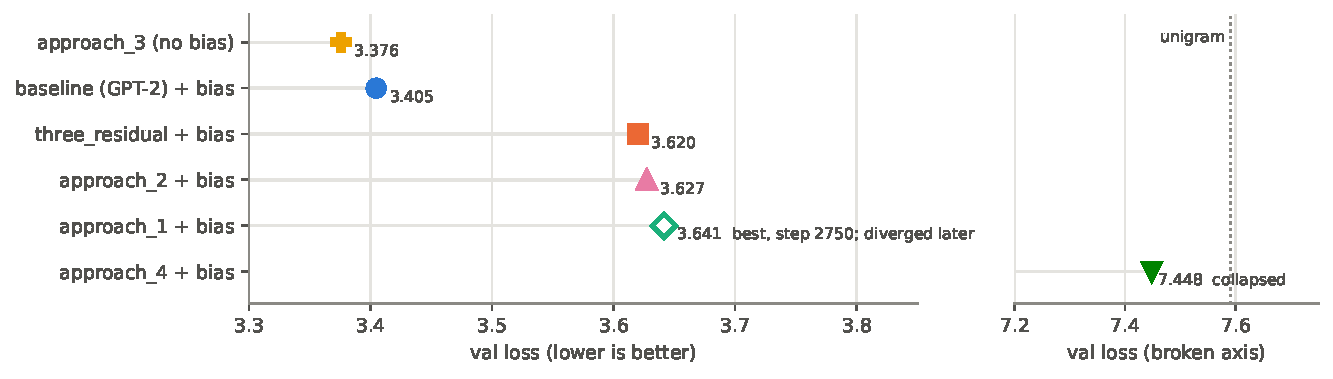
\includegraphics[width=\linewidth]{figures/fig_final_loss.pdf}
\caption{Validation loss after 2.5B OpenWebText tokens on the full 20M-token split. \aone{} (open diamond) did not
finish: its value is the best 4M-token evaluation, at step \BestAOneStep{}, before it diverged. The right panel is
a broken axis for the collapsed \afour{}; the dotted line is the unigram model.}
\label{fig:final}
\end{figure}

\begin{itemize}
\item \textbf{\atwo{}: rescued.} It trains stably to \FinalATwo{}, level with \tr{} (\FinalTR{}) and
\GapATwo{} nats behind GPT-2 trained with the same bias (\FinalBase{}). Without the bias it stays at the unigram
level (\NoBiasTwo{} at step 500).
\item \textbf{\aone{}: rescued, then unstable.} It learned fastest of the new variants: at step 2500 it was
only 0.10 nats behind the control. From step $\sim$2750 its gradient norm grew from \GnAOneEarly{} to
\GnAOneLate{} (medians), and around step 3600 the loss blew up. Best value \BestAOne{} at step
\BestAOneStep{}; the run was stopped at step 3690.
\item \textbf{\afour{}: not rescued.} It trained well while the bias was on (\AFourAtSevenFifty{} at step 750,
ahead of \atwo{}), became unstable as the bias fell below about 2, and collapsed within 250 steps of the bias
reaching 0 (\AFourAtOneTwoFiveK{} at step 1250). It ended at \FinalAFour{}, near the unigram loss.
\item \textbf{Why \afour{} fails is not that it cannot learn the right attention.} Checkpoints show that its own
query-key logits learn to attend to the token itself as fast as \atwo{}'s do (mean self-weight with the bias
removed: \SzAFourSevenFifty{} vs.\ \SzATwoSevenFifty{} at step 750). It then loses this attention in one burst
after step 1000, while its gradient norm is far above the clipping threshold.
\item \textbf{The surviving models attend mostly to themselves.} With the bias at 0, \atwo{} puts a mean weight of
\SelfATwo{} on the token itself (\SelfHeadsATwo{} of 144 heads above 0.5); \tr{}: \SelfTR{}; GPT-2: \SelfBase{}.
\end{itemize}

%==============================================================================
\section{Setup}

\begin{center}\small
\begin{tabularx}{\linewidth}{lX}
\toprule
Data & OpenWebText, GPT-2 BPE; train 2.69B tokens, validation 20M tokens (same split as the 2026-10-19 report) \\
Budget & 2.5B tokens: 4768 steps $\times$ 524{,}288 tokens \\
Optimizer & AdamW, $\beta=(0.9, 0.95)$, weight decay 0.1 (matrices only), gradient clip 1.0 \\
Learning rate & linear warmup over 250 steps to $6\times10^{-4}$, cosine decay to $6\times10^{-5}$ \\
Batch & 16 micro-batches of $32\times1024$ tokens; bf16 autocast; \code{torch.compile}; one H100 per run \\
Bias schedule & $b(t) = 8\max(0, 1 - t/1000)$ on every head's self logit, a non-learned buffer \\
Seed and order & seed 1337 and the same sequential data order in every run \\
Evaluation & 4M validation tokens every 250 steps; the full 20M tokens at the end \\
\bottomrule
\end{tabularx}
\end{center}

All numbers are on the same OpenWebText validation split and are comparable with the 2026-10-19 report (the
\tr{}, baseline and approach\_3 runs shown here are those runs). They are not comparable with the FineWeb-Edu
numbers of the 2026-10-15/16 reports. The unigram model scores \Unigram{}.

\paragraph{Runs in this report.}
\begin{center}\footnotesize
\begin{tabularx}{\linewidth}{p{4.2cm}p{3.6cm}X}
\toprule
Run & Purpose & Directory under \code{runs/openwebtext/} \\
\midrule
\aone{}, \atwo{}, \afour{} + bias & main runs, 2.5B tokens & \code{approach\_\{1,2,4\}\_diag8\_anneal1000} \\
\aone{}, \atwo{}, \afour{}, no bias & collapse reference, 500 steps & \code{approach\_\{1,2,4\}\_nobias\_s500} \\
\atwo{}, \afour{} + bias, repeated & checkpoints at steps 500--1250 & \code{approach\_\{2,4\}\_diag8\_repro} \\
baseline + bias, \tr{} + bias, approach\_3 & references (2026-10-19) & \code{baseline\_diag8\_anneal1000}, \code{tr\_diag8\_anneal1000}, \code{approach\_3} \\
\bottomrule
\end{tabularx}
\end{center}
The main runs keep only their latest checkpoint, so the checkpoints around the end of annealing come from the
repeated runs: same seed, data order and settings, stopped at step 1250. They reproduce the main runs closely,
though not bit for bit (\atwo{} at step 250: 6.12 vs.\ 6.08; \afour{} at step 1000: 5.16 vs.\ 5.06), and the
repeated \afour{} collapses at the same point.

%==============================================================================
\section{Structure}\label{sec:structure}

\subsection{The blocks}
For head $h$ (12 heads, $d = 64$), $X_h$ is the head's $d$-dimensional slice of the raw residual stream $X$ (before
$\mathrm{LN}_1$), and $Q_h$, $K_h$, $V_h$ are computed from $\mathrm{LN}_1(X)$ as in GPT-2. During pretraining the
causal attention matrix is
\[
A_h = \mathrm{softmax}\!\Big(\tfrac{1}{\sqrt d}\,Q_hK_h^\top + b\,I + \text{mask}\Big),
\]
and from step 1000 on $b = 0$, so every model is exactly as defined below. Only the attention sublayer differs;
the MLP sublayer is standard in all variants, $X^{(\ell+1)} = X' + \mathrm{MLP}(\mathrm{LN}_2(X'))$.
\begin{align}
\text{baseline (GPT-2):}\quad & X' = X + \cat[A_hV_h]\,W_O + b_O \\
\text{\aone{}:}\quad & Y = \cat[A_h(V_h + X_h)], \qquad X' = Y W_O + b_O + Y \label{eq:a1}\\
\text{\atwo{}:}\quad & Y = \mathrm{LN}\big(\cat[A_h(V_h + X_h)]\big), \qquad X' = Y W_O + b_O + Y \label{eq:a2}\\
\text{\afour{}:}\quad & X' = \cat[A_hV_h]\,W_O + b_O + \cat[A_hX_h] \label{eq:a4}
\end{align}
The LayerNorm in \atwo{} has no affine parameters. All three new variants have exactly GPT-2's parameters (124{,}475{,}904): they reuse $W_Q$, $W_K$, $W_V$ and
$W_O$, and only re-route $X$. For reference, \tr{} is $Z_h = (I + A_h)X_h$, $Y = \cat[Z_h(I + W_{vh})]$,
$X' = Y(I + W_O) + b_O$, and approach\_3 is $X' = X + \cat[A_h(V_h+X_h)]W_O + b_O$.

\begin{figure}[H]
\centering
\resizebox{\linewidth}{!}{%
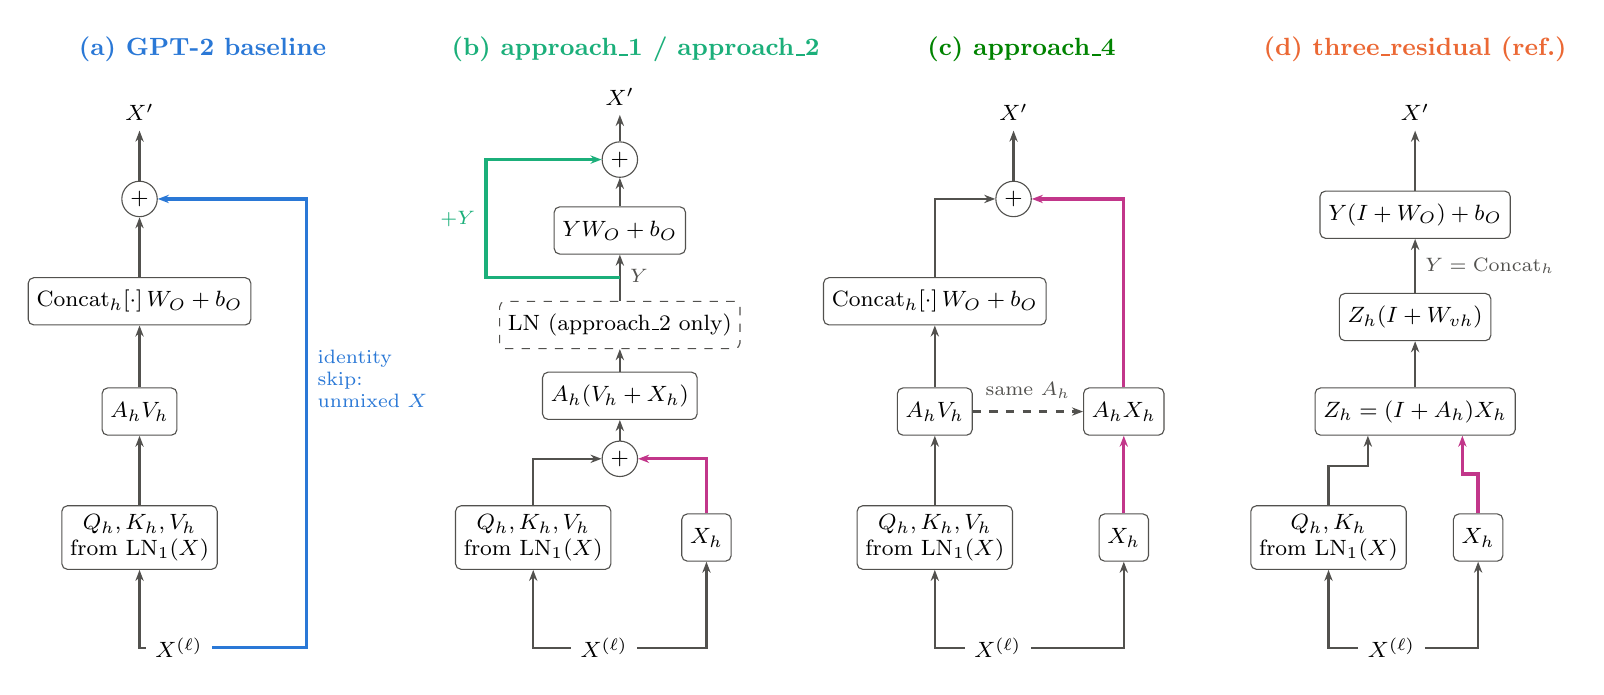
\begin{tikzpicture}[
  font=\footnotesize,
  box/.style={draw=ink2, rounded corners=2pt, minimum height=0.6cm, align=center, fill=white, inner sep=3pt},
  dbox/.style={box, dashed},
  op/.style={draw=ink2, circle, inner sep=0.5pt, minimum size=0.45cm, fill=white},
  arr/.style={-{Stealth[length=4pt]}, ink2, thick},
  skip/.style={-{Stealth[length=4pt]}, cbase, very thick},
  mix/.style={-{Stealth[length=4pt]}, cmix, very thick},
  yskip/.style={-{Stealth[length=4pt]}, cone, very thick},
]
% ---------------- (a) baseline ----------------
\begin{scope}[shift={(0,0)}]
  \node[font=\small\bfseries, text=cbase] at (0.3,7.6) {(a) GPT-2 baseline};
  \node (x) at (0,0) {$X^{(\ell)}$};
  \node[box] (qkv) at (-0.5,1.4) {$Q_h,K_h,V_h$\\from $\mathrm{LN}_1(X)$};
  \node[box] (av) at (-0.5,3.0) {$A_hV_h$};
  \node[box] (wo) at (-0.5,4.4) {$\cat[\cdot]\,W_O + b_O$};
  \node[op] (add) at (-0.5,5.7) {$+$};
  \node (out) at (-0.5,6.8) {$X'$};
  \draw[arr] (x) -| (qkv.south);
  \draw[arr] (qkv) -- (av); \draw[arr] (av) -- (wo); \draw[arr] (wo) -- (add); \draw[arr] (add) -- (out);
  \draw[skip] (x.east) -- ++(1.2,0) |- node[pos=0.3, right, align=left, font=\scriptsize] {identity\\skip:\\unmixed $X$} (add.east);
\end{scope}
% ---------------- (b) approach_1 / approach_2 ----------------
\begin{scope}[shift={(5.4,0)}]
  \node[font=\small\bfseries, text=cone] at (0.4,7.6) {(b) approach\_1 / approach\_2};
  \node (x) at (0,0) {$X^{(\ell)}$};
  \node[box] (qkv) at (-0.9,1.4) {$Q_h,K_h,V_h$\\from $\mathrm{LN}_1(X)$};
  \node[box] (xh) at (1.3,1.4) {$X_h$};
  \node[op] (vx) at (0.2,2.4) {$+$};
  \node[box] (a) at (0.2,3.2) {$A_h(V_h + X_h)$};
  \node[dbox] (ln) at (0.2,4.1) {$\mathrm{LN}$ (\atwo{} only)};
  \node[box] (wo) at (0.2,5.3) {$Y W_O + b_O$};
  \node[op] (add) at (0.2,6.2) {$+$};
  \node (out) at (0.2,7.0) {$X'$};
  \draw[arr] (x) -| (qkv.south); \draw[arr] (x) -| (xh.south);
  \draw[arr] (qkv.north) |- (vx.west); \draw[mix] (xh.north) |- (vx.east);
  \draw[arr] (vx) -- (a); \draw[arr] (a) -- (ln); \draw[arr] (ln) -- node[pos=0.55, right, font=\scriptsize]{$Y$} (wo);
  \draw[arr] (wo) -- (add); \draw[arr] (add) -- (out);
  \draw[yskip] ($(ln.north)!0.5!(wo.south)$) -- ++(-1.7,0) |- node[pos=0.25, left, font=\scriptsize]{$+Y$} (add.west);
\end{scope}
% ---------------- (c) approach_4 ----------------
\begin{scope}[shift={(10.4,0)}]
  \node[font=\small\bfseries, text=cfour] at (0.3,7.6) {(c) approach\_4};
  \node (x) at (0,0) {$X^{(\ell)}$};
  \node[box] (qkv) at (-0.8,1.4) {$Q_h,K_h,V_h$\\from $\mathrm{LN}_1(X)$};
  \node[box] (xh) at (1.6,1.4) {$X_h$};
  \node[box] (av) at (-0.8,3.0) {$A_hV_h$};
  \node[box] (ax) at (1.6,3.0) {$A_hX_h$};
  \node[box] (wo) at (-0.8,4.4) {$\cat[\cdot]\,W_O + b_O$};
  \node[op] (add) at (0.2,5.7) {$+$};
  \node (out) at (0.2,6.8) {$X'$};
  \draw[arr] (x) -| (qkv.south); \draw[arr] (x) -| (xh.south);
  \draw[arr] (qkv) -- (av); \draw[mix] (xh) -- (ax);
  \draw[arr, dashed] (av.east) -- node[above=1pt, font=\scriptsize]{same $A_h$} (ax.west);
  \draw[arr] (av) -- (wo); \draw[arr] (wo.north) |- (add.west); \draw[mix] (ax.north) |- (add.east);
  \draw[arr] (add) -- (out);
\end{scope}
% ---------------- (d) three_residual ----------------
\begin{scope}[shift={(15.4,0)}]
  \node[font=\small\bfseries, text=ctr] at (0.3,7.6) {(d) three\_residual (ref.)};
  \node (x) at (0,0) {$X^{(\ell)}$};
  \node[box] (qk) at (-0.8,1.4) {$Q_h,K_h$\\from $\mathrm{LN}_1(X)$};
  \node[box] (xh) at (1.1,1.4) {$X_h$};
  \node[box] (z) at (0.3,3.0) {$Z_h=(I + A_h)X_h$};
  \node[box] (v) at (0.3,4.2) {$Z_h(I + W_{vh})$};
  \node[box] (o) at (0.3,5.5) {$Y(I + W_O) + b_O$};
  \node (out) at (0.3,6.8) {$X'$};
  \draw[arr] (x) -| (qk.south); \draw[arr] (x) -| (xh.south);
  \draw[arr] (qk.north) -- ++(0,0.5) -| ([xshift=-6mm]z.south); \draw[mix] (xh.north) -- ++(0,0.5) -| ([xshift=6mm]z.south);
  \draw[arr] (z) -- (v); \draw[arr] (v) -- node[right, font=\scriptsize]{$Y=\cat$} (o); \draw[arr] (o) -- (out);
\end{scope}
\end{tikzpicture}}
\caption{Attention sublayers. Blue: GPT-2's identity skip, which carries each token's state to the next layer
unmixed. Magenta: the raw stream $X_h$ entering the attention average $A_h$ at full scale. Green: the skip
around $W_O$ in \aone{}/\atwo{}, which carries $Y$, itself already averaged by $A_h$. In \aone{}, \atwo{} and
\afour{}, every path from $X^{(\ell)}$ to $X'$ passes through some $A_h$; none has an unmixed copy of $X$.
In \tr{} (d) the identity inside $(I + A_h)$ does carry $X_h$ unmixed, but at the same scale as $A_hX_h$.}
\label{fig:arch}
\end{figure}

\subsection{Expanding the outputs}
Dropping the biases and writing each output as a sum of terms shows what reaches the next layer:
\begin{center}\footnotesize
\renewcommand{\arraystretch}{1.25}
\begin{tabular}{lll}
\toprule
Variant & Attention sublayer output $X'$ & Unmixed $X$? \\
\midrule
baseline & $X + \cat[A_hV_h]W_O$ & yes \\
approach\_3 & $X + \cat[A_hV_h]W_O + \cat[A_hX_h]W_O$ & yes \\
\tr{} & $\cat\big[(X_h + A_hX_h)(I + W_{vh})\big](I + W_O)$ & yes$^{*}$ \\
\midrule
\aone{} & $\cat[A_hX_h] + \cat[A_hV_h] + \cat[A_hX_h]W_O + \cat[A_hV_h]W_O$ & no \\
\atwo{} & $\mathrm{LN}\big(\cat[A_hX_h + A_hV_h]\big)\,(I + W_O)$ & no \\
\afour{} & $\cat[A_hX_h] + \cat[A_hV_h]W_O$ & no \\
\bottomrule
\end{tabular}\\[2pt]
{\scriptsize $^{*}$ at the same scale as the averaged term $A_hX_h$}
\end{center}

\begin{itemize}
\item \textbf{At initialization the terms differ a lot in size.} $V_h$ comes from $\mathrm{LN}_1(X)$, which has
unit scale, while the token and position embeddings have standard deviation 0.02; and $W_O$ shrinks whatever passes
through it by about 10$\times$. Measured norms at layer 0 (4 validation sequences, identical for the three
variants):
\begin{center}\footnotesize
\begin{tabular}{lccccc}
\toprule
 & $X$ & $\cat[A_hX_h]$ & $\cat[A_hV_h]$ & $\cat[A_hX_h]W_O$ & $\cat[A_hV_h]W_O$ \\
\midrule
no bias & 49 & 5 & 90 & 1 & 10 \\
$b = 8$ & 49 & 41 & 801 & 5 & 91 \\
\bottomrule
\end{tabular}
\end{center}
So the variants differ in how fresh content enters the stream: \aone{} and \atwo{} add the averaged values
$\cat[A_hV_h]$ at full scale in every layer, \afour{} only through $W_O$. By layer 11 (with $b = 8$) the stream has
grown to a norm of 1785 in \aone{} and 1732 in \atwo{}, but only 388 in \afour{}.
\item \textbf{Every term is an average over the prefix.} With near-uniform attention all of them are close to the
prefix mean (the random values largely cancel, which is why $\cat[A_hV_h]$ is 90 rather than 801), and 12 layers
of this make every position alike (Section~\ref{sec:init}). With $b = 8$, $A_h \approx I$, so
$A_hX_h \approx X_h$ and $A_hV_h \approx V_h$: the bias temporarily turns the averages into per-token terms and
stands in for the missing identity skip.
\item \textbf{\aone{} contains \afour{}.} \aone{} has both of \afour{}'s terms and adds two more, $\cat[A_hV_h]$
(the averaged values at full scale, with no $W_O$) and $\cat[A_hX_h]W_O$. So the two variants differ only by
extra terms; neither has a path the other lacks around the attention.
\item \textbf{\atwo{}} is \aone{} with the attention output normalized before $W_O$ and before the skip, so the
scale of $Y$ is fixed regardless of the scale of $X$.
\end{itemize}
The 2026-10-16 rule (``a variant trains only if each token's state has an unmixed path to the next layer'')
classified all three as untrainable. The results below show that this rule describes initialization, not the
architecture: \aone{} and \atwo{} train with no unmixed path once they start from a good point.

%==============================================================================
\section{Initialization}\label{sec:init}

The probe runs the freshly initialized model on 8 validation sequences and records, after every layer, the
residual stream's \emph{distance from rank 1}, $\lVert X - \bar X\rVert / \lVert X\rVert$, where $\bar X$ repeats
the mean over positions (positions below 64 skipped). In every earlier case a layer-11 value of about 0.15 or
less predicted collapse.

\begin{figure}[H]
\centering
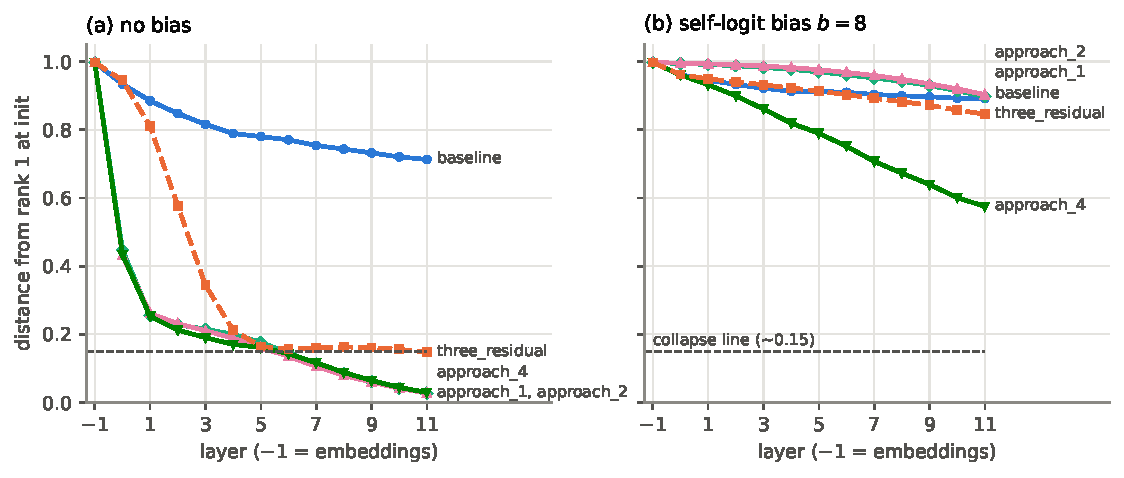
\includegraphics[width=\linewidth]{figures/fig_init_probe.pdf}
\caption{Distance from rank 1 at initialization. (a) Without the bias, \aone{}, \atwo{} and \afour{} lose almost
all position-specific information by layer 5 and end at about 0.03, below even \tr{}. (b) With $b=8$ all
variants stay far above the collapse line. \afour{} decays fastest (\ProbeEightFour{} at layer 11), but it is
still well clear of the line.}
\label{fig:probe}
\end{figure}

\begin{center}\small
\begin{tabular}{lccc}
\toprule
Layer-11 distance from rank 1 at init & no bias & $b = 8$ & val loss at step 500, no bias \\
\midrule
baseline & \ProbeBase{} & 0.892 & --- \\
\aone{} & \ProbeZeroOne{} & \ProbeEightOne{} & \NoBiasOne{} \\
\atwo{} & \ProbeZeroTwo{} & \ProbeEightTwo{} & \NoBiasTwo{} \\
\afour{} & \ProbeZeroFour{} & \ProbeEightFour{} & \NoBiasFour{} \\
\bottomrule
\end{tabular}
\end{center}

\begin{figure}[H]
\centering
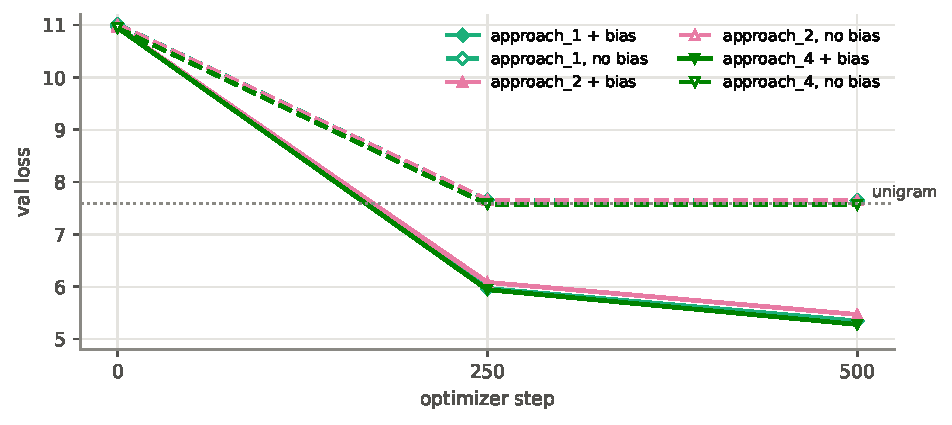
\includegraphics[width=0.78\linewidth]{figures/fig_nobias.pdf}
\caption{First 500 steps with and without the bias. Without it (dashed, open markers), all three variants
flatten at the unigram loss within 250 steps on OpenWebText too, confirming the FineWeb-Edu result on this data.
With it (solid) they learn like the healthy models. (\aone{} + bias is hidden under \afour{} + bias.)}
\label{fig:nobias}
\end{figure}

%==============================================================================
\section{Pretraining}

\begin{figure}[H]
\centering
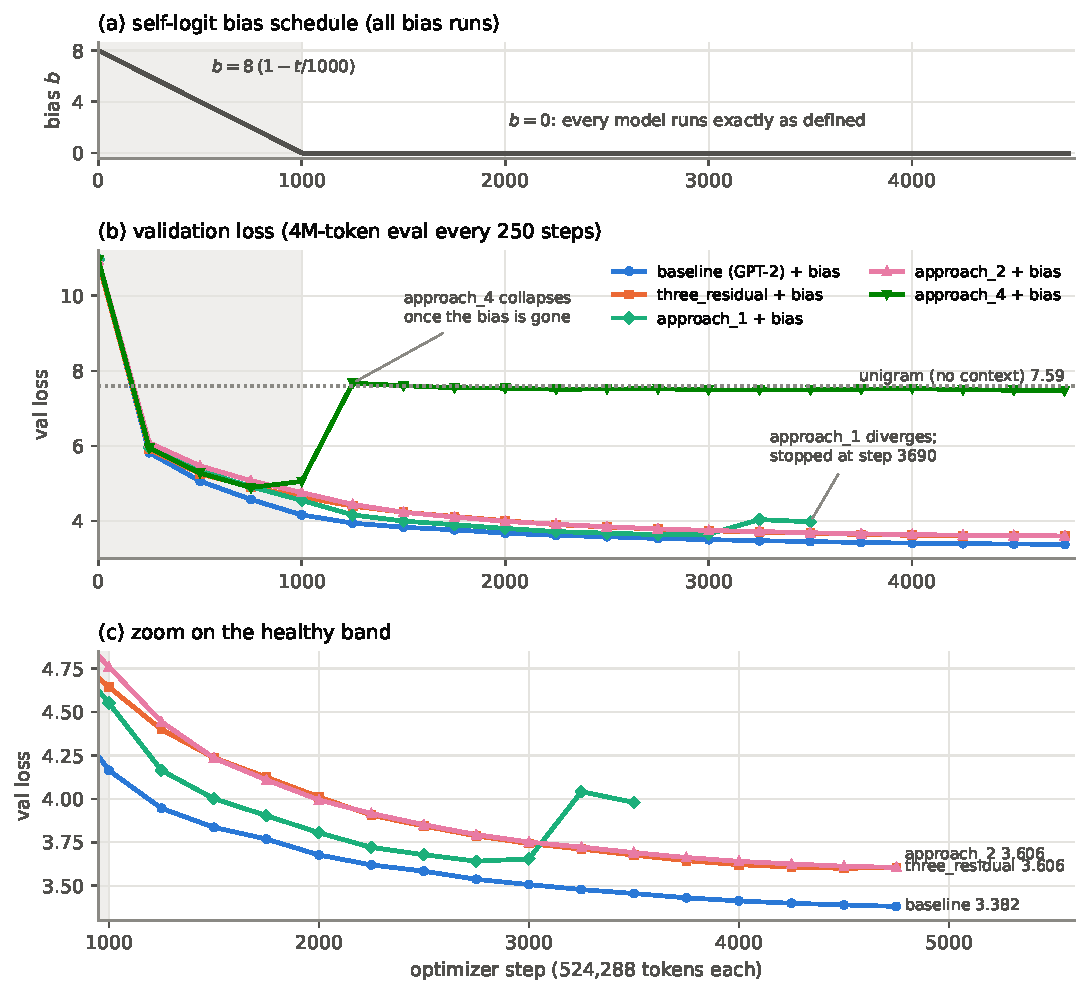
\includegraphics[width=0.96\linewidth]{figures/fig_training.pdf}
\caption{(a) Bias schedule; the shaded band marks steps 0--1000, while the bias is non-zero. (b) Validation loss
of all bias runs. (c) Zoom on the healthy band, steps 1000--4750; labels give the last 4M-token value (the
final 20M-token values are in Figure~\ref{fig:final}).}
\label{fig:training}
\end{figure}

\begin{figure}[H]
\centering
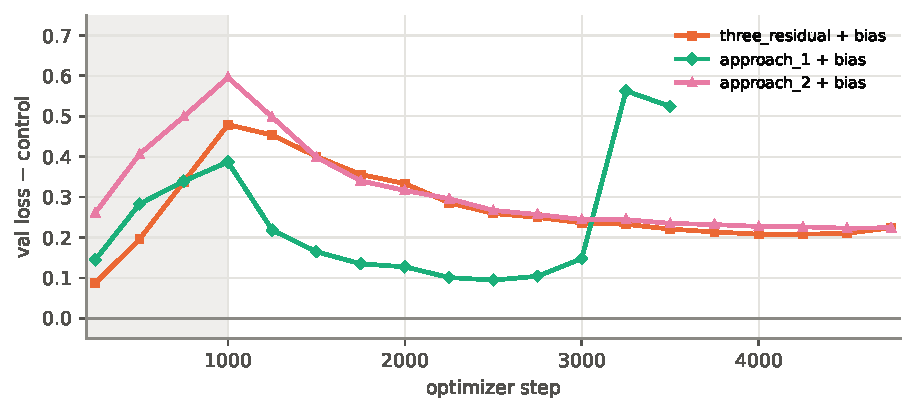
\includegraphics[width=0.8\linewidth]{figures/fig_gap.pdf}
\caption{Validation loss minus the GPT-2 control at the same step. All three healthy variants lag most at
step 1000, when the bias reaches 0, and then close in. \aone{} closes fastest, to 0.10 nats at step 2500, before
it diverges. \atwo{} and \tr{} follow almost the same curve and both settle near 0.22.}
\label{fig:gap}
\end{figure}

\begin{center}\footnotesize
\begin{tabular}{lccccc}
\toprule
Val loss & step 750 ($b=2$) & step 1000 ($b=0$) & step 1250 & step 2500 & final (20M) \\
\midrule
baseline + bias & 4.58 & \BaseAtOneK{} & 3.95 & 3.58 & \FinalBase{} \\
\tr{} + bias & 4.91 & \TRAtOneK{} & 4.40 & 3.84 & \FinalTR{} \\
\aone{} + bias & 4.92 & \AOneAtOneK{} & \AOneAtOneTwoFiveK{} & 3.68 & diverged (best \BestAOne{}) \\
\atwo{} + bias & 5.07 & \ATwoAtOneK{} & \ATwoAtOneTwoFiveK{} & 3.85 & \FinalATwo{} \\
\afour{} + bias & \AFourAtSevenFifty{} & \AFourAtOneK{} & \AFourAtOneTwoFiveK{} & 7.52 & \FinalAFour{} \\
\bottomrule
\end{tabular}
\end{center}

\paragraph{Throughput.} The bias needs an additive attention mask, which rules out PyTorch's fastest attention
kernel. \atwo{} trained at \TokATwo{}k tokens/s. \afour{} needs two attention calls when the bias is on
(Section~\ref{sec:code}) and ran at \TokAFour{}k tokens/s.

%==============================================================================
\section{Stability}

\begin{figure}[H]
\centering
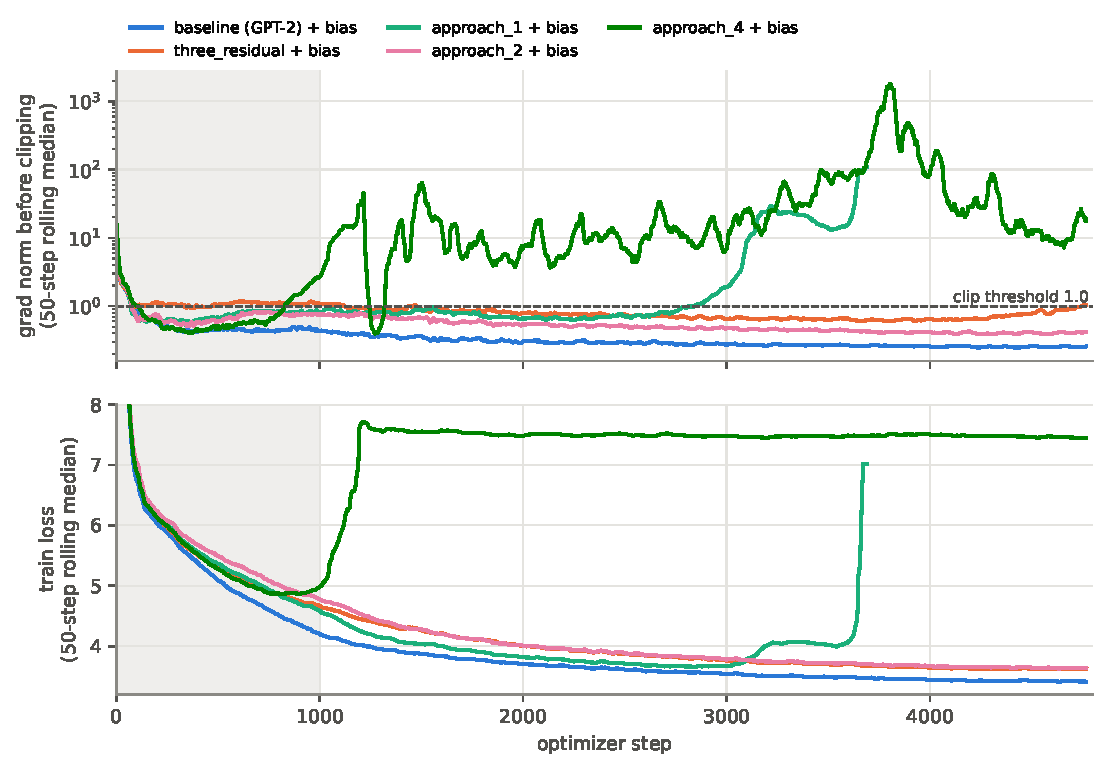
\includegraphics[width=0.96\linewidth]{figures/fig_grad_norm.pdf}
\caption{Gradient norm before clipping (top, log scale) and training loss (bottom), both as 50-step rolling
medians. The control, \tr{} and \atwo{} stay below the clip threshold for the whole run. \afour{} rises above it
from step $\sim$800 and \aone{} from step $\sim$2900; each loss blows up after its gradient norm has risen by
about an order of magnitude.}
\label{fig:gn}
\end{figure}

\begin{center}\small
\begin{tabular}{lc}
\toprule
Median gradient norm (pre-clip) & steps 3000--3500 \\
\midrule
baseline + bias & \GnBaseLate{} \\
\tr{} + bias & \GnTRLate{} \\
\atwo{} + bias & \GnATwoLate{} \\
\aone{} + bias & \GnAOneLate{} (steps 1000--2500: \GnAOneEarly{}) \\
\bottomrule
\end{tabular}
\end{center}

\subsection{\afour{} at the end of annealing}

\begin{figure}[H]
\centering
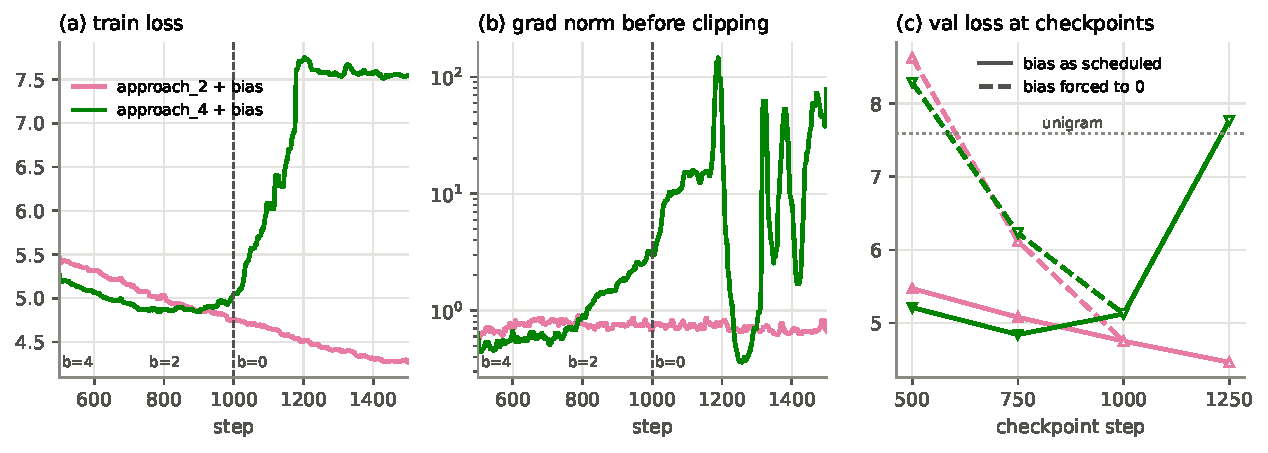
\includegraphics[width=\linewidth]{figures/fig_anneal_end.pdf}
\caption{Steps 500--1500 for \atwo{} and \afour{}. (a) Training loss and (b) gradient norm, 20-step rolling
medians; the bias values are marked at the bottom. (c) Validation loss (2M tokens) of the checkpoints from the
repeated runs, with the bias at its scheduled value (solid) and forced to 0 (dashed). Where the two lines meet,
the model no longer needs the bias.}
\label{fig:anneal}
\end{figure}

\begin{center}\footnotesize
\setlength{\tabcolsep}{4pt}
\begin{tabular}{lcccccc}
\toprule
 & \multicolumn{3}{c}{\atwo{}} & \multicolumn{3}{c}{\afour{}} \\
\cmidrule(lr){2-4}\cmidrule(lr){5-7}
Checkpoint & val, bias on & val, $b=0$ & self-weight, $b=0$ & val, bias on & val, $b=0$ & self-weight, $b=0$ \\
\midrule
step 750 ($b=2$) & \VbATwoSevenFifty{} & \VzATwoSevenFifty{} & \SzATwoSevenFifty{} & \VbAFourSevenFifty{} & \VzAFourSevenFifty{} & \SzAFourSevenFifty{} \\
step 1000 ($b\approx0$) & \VbATwoOneK{} & \VzATwoOneK{} & \SzATwoOneK{} & \VbAFourOneK{} & \VzAFourOneK{} & \SzAFourOneK{} \\
step 1250 ($b=0$) & 4.46 & 4.46 & 0.85 & 7.76 & 7.76 & 0.06 \\
\bottomrule
\end{tabular}
\end{center}

\begin{figure}[H]
\centering
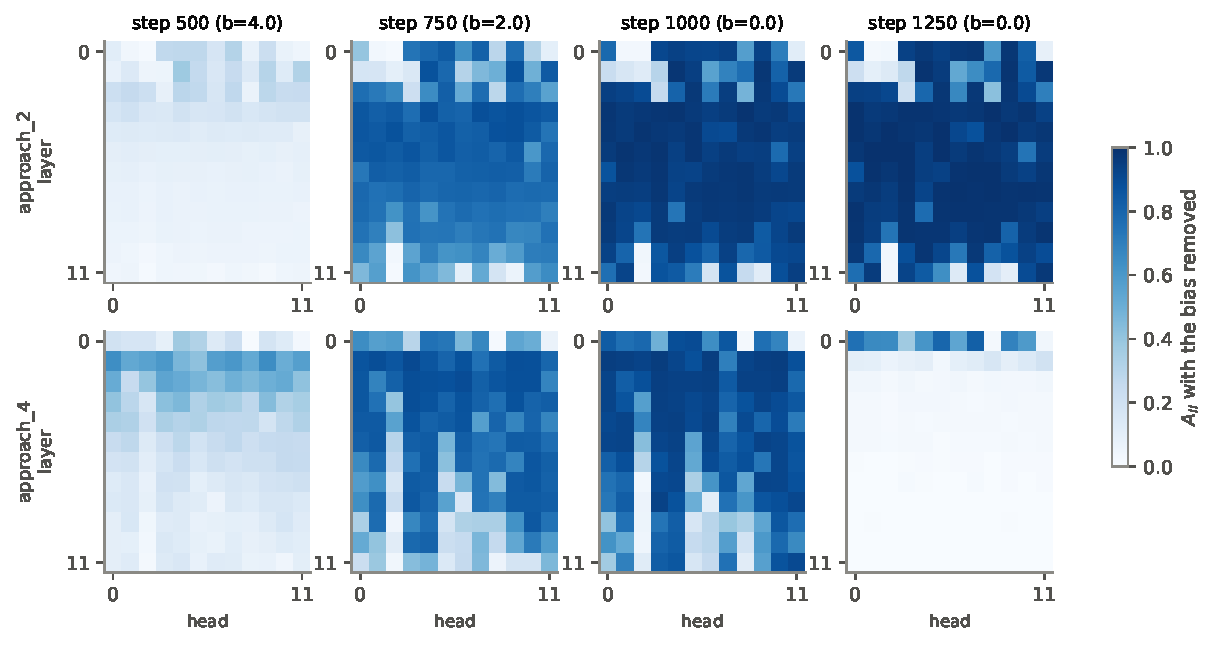
\includegraphics[width=0.9\linewidth]{figures/fig_selfweight_learned.pdf}
\caption{Self-weight $A_{ii}$ of every head (rows: layers 0--11, columns: heads) computed from the learned
query-key logits alone, i.e.\ with the bias removed. Both variants learn self-attention at about the same pace
between steps 500 and 1000. \afour{}'s deep layers learn less of it (layers 6--11: 0.62 at step 1000 vs.\ 0.86
for \atwo{}). Between steps 1000 and 1250 \afour{} loses almost all of it.}
\label{fig:sw-learned}
\end{figure}

What the checkpoints show:
\begin{itemize}
\item \textbf{Both variants take over the bias's job.} At step 500 neither works without the bias (validation loss
above the unigram level when it is removed). By step 1000 both have learned query-key logits that put most
attention on the token itself, and removing the remaining bias changes nothing.
\item \textbf{\afour{} starts degrading before the bias is gone.} Its gradient norm leaves the clip threshold at
about step 800 ($b \approx 1.6$; median \GnAFourMid{} at steps 650--700 vs.\ \GnAFourEnd{} at 1000--1050), and
its loss is higher at step 1000 than at step 750, although it no longer depends on the bias at step 1000.
\item \textbf{The collapse is a loss of the learned self-attention.} Between steps 1000 and 1250 the self-weight
falls from \SzAFourOneK{} to 0.06 (heads above 0.5: 119 $\to$ 9), and the residual stream becomes rank 1 (layer-11
distance 0.004). The model ends where the unbiased model starts, and it never recovers: its attention afterwards
is sharp but shared across queries, the pattern seen in the 2026-10-16 \afour{} run.
\end{itemize}
So the bias fixes \afour{}'s starting point, as it does for the other variants, but \afour{} cannot hold the state
it reaches. Why it is unstable and \atwo{} is not has not been established. Candidates: \atwo{}'s LayerNorm fixes
the scale of $Y$; \aone{} and \atwo{} add fresh, full-scale per-token content $\cat[A_hV_h]$ in every layer, while
\afour{}'s update is almost a pure average of the existing stream $X$ (its values enter only through $W_O$), so an
error in $A_h$ is not diluted by anything new.

\subsection{\aone{}'s late divergence}
\aone{} was healthy for 2000 steps after the bias reached 0, and better than \atwo{} and \tr{}. Its gradient
norm started rising at about step 2750, crossed the clip threshold near step 2900 and reached medians of
\GnAOneLate{} after step 3000, with single steps above 300. Validation loss went from \AOneAtThreeK{} at step 3000
to \AOneAtThreeQK{} at step 3250, and the training loss climbed above 5 by step 3630. The step-3000 checkpoint is
kept (\code{ckpt\_step3000.pt}). Unlike \atwo{}, \aone{} has no normalization on $Y$, and $Y$ feeds the stream at full
scale through the skip around $W_O$; a growing stream scale is the first thing to check. A rerun with a lower
peak learning rate would show whether this is a learning-rate problem or a property of the block.

%==============================================================================
\section{The trained models}

All numbers in this section are averages over 8 validation sequences and query positions $\ge 64$; heatmaps
show the first 48 tokens of one sequence. The bias is 0 in every model shown.

\begin{figure}[H]
\centering
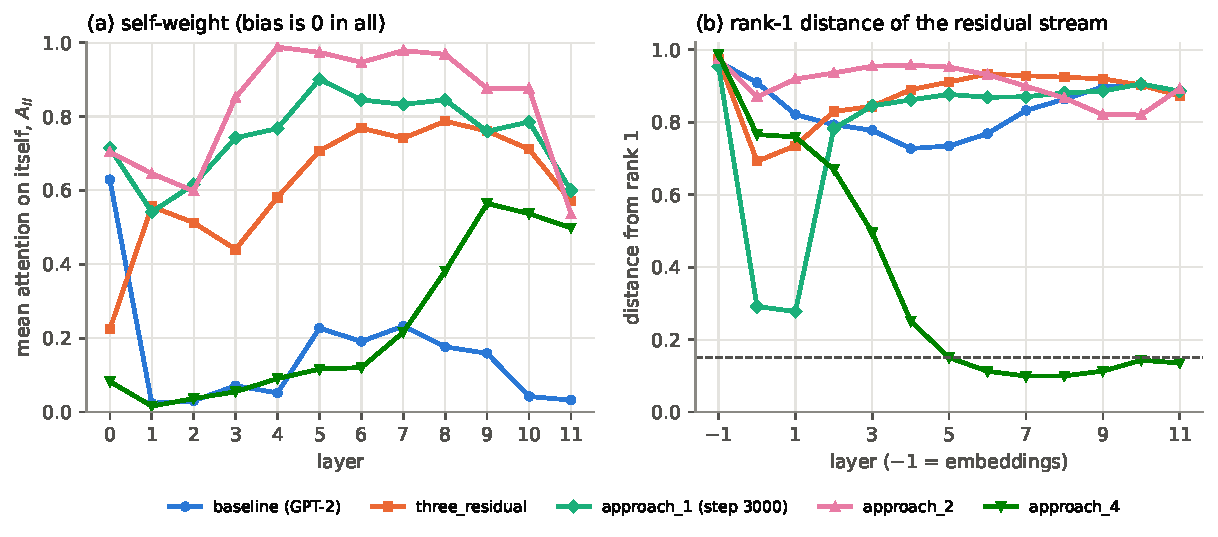
\includegraphics[width=\linewidth]{figures/fig_trained_diag.pdf}
\caption{(a) Mean attention on the token itself, per layer. (b) Distance from rank 1 of the residual stream.
\aone{} is shown at step 3000, its last checkpoint before the divergence.}
\label{fig:trained}
\end{figure}

\begin{center}\small
\begin{tabular}{lccc}
\toprule
 & mean $A_{ii}$ & heads with $A_{ii} > 0.5$ & layer-11 distance from rank 1 \\
\midrule
baseline + bias & \SelfBase{} & \SelfHeadsBase{} / 144 & \RankBase{} \\
\tr{} + bias & \SelfTR{} & \SelfHeadsTR{} / 144 & \RankTR{} \\
\aone{} + bias (step 3000) & \SelfAOne{} & \SelfHeadsAOne{} / 144 & \RankAOne{} \\
\atwo{} + bias & \SelfATwo{} & \SelfHeadsATwo{} / 144 & \RankATwo{} \\
\afour{} + bias (collapsed) & \SelfAFour{} & \SelfHeadsAFour{} / 144 & \RankAFour{} \\
\bottomrule
\end{tabular}
\end{center}

\begin{figure}[H]
\centering
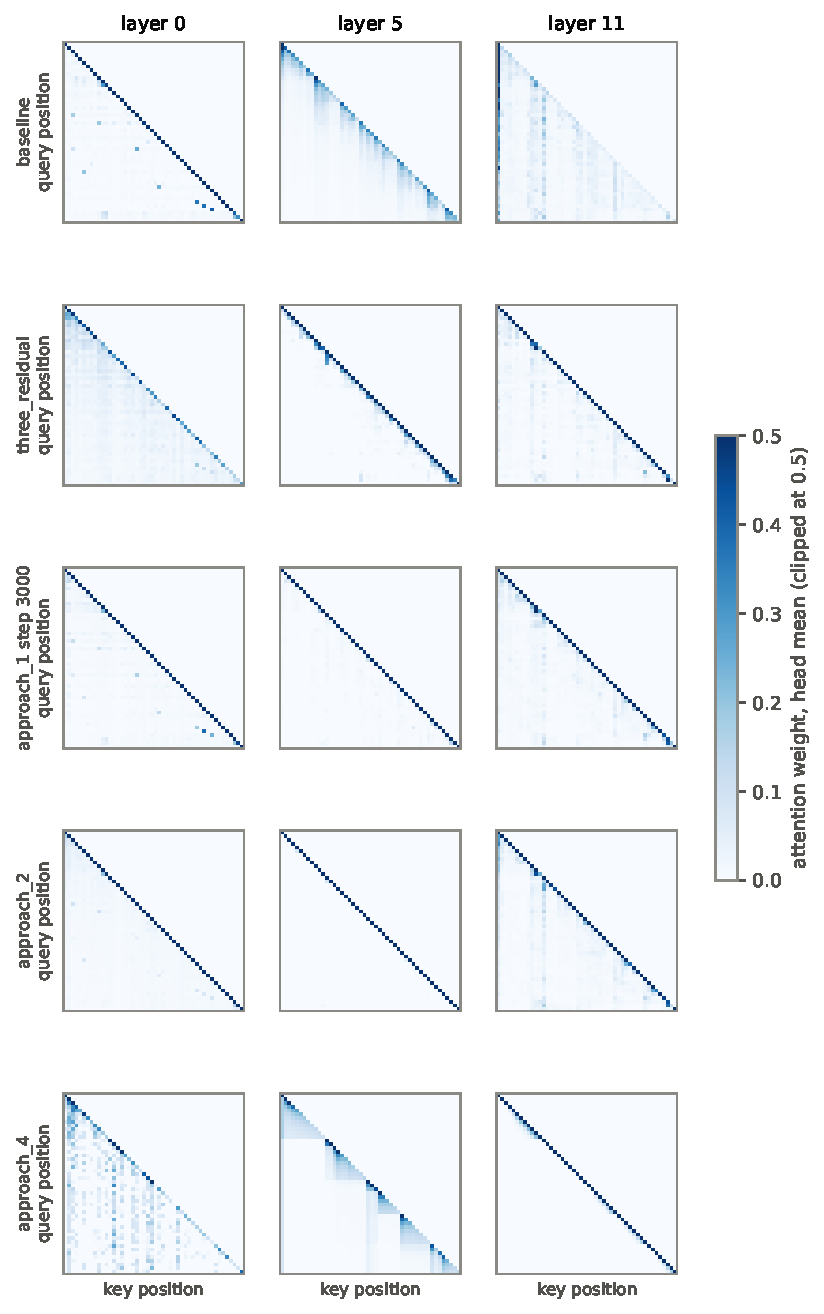
\includegraphics[width=0.56\linewidth]{figures/fig_attention_trained.pdf}
\caption{Attention averaged over heads at layers 0, 5 and 11. \aone{} and \atwo{} are almost pure self-attention
at every depth, with a few weak stripes on earlier tokens. The GPT-2 control shows the usual patterns
(previous tokens, a column on the first token). The collapsed \afour{} has block-shaped attention in layer 5:
queries in a block all read the same position.}
\label{fig:attn}
\end{figure}

\begin{itemize}
\item \textbf{The surviving variants keep each token's state by attending to itself.} \atwo{} puts 0.95--0.99 on
the token itself in layers 4--8. This is the same strategy \tr{} learned, carried further: without an identity
skip, $A_h \approx I$ is the only way to keep a token's own state dominant.
\item \textbf{Little attention is left for moving information.} Only \the\numexpr144-\SelfHeadsATwo\relax{} of
\atwo{}'s 144 heads put less than half their weight on the token itself (control: \the\numexpr144-\SelfHeadsBase\relax{}).
That \atwo{} still reaches \FinalATwo{} means a small amount of off-diagonal attention, plus the MLPs, does most of
the work. This is also a plausible reason for the remaining 0.22-nat gap, but it has not been tested.
\item \textbf{\aone{}'s stream briefly narrows.} At step 3000 its distance from rank 1 drops to 0.29 after layers
0 and 1 and recovers by layer 2 (Figure~\ref{fig:trained}b). No other healthy model shows this.
\end{itemize}

%==============================================================================
\section{Code changes}\label{sec:code}
\begin{itemize}
\item \code{train/gpt2\_torch.py}: the self-logit bias now also applies to \afour{} and approach\_5 (it was blocked
by an assert). Under \code{torch.compile}, the original single attention call on the concatenated
$[V_h \mid X_h]$ (value width 128, query width 64) with an additive mask gave NaN gradients at step 0, while eager
mode was fine. When the bias is on, $A_hV_h$ and $A_hX_h$ are now computed with two separate attention calls;
the compiled run then matches eager mode exactly. Without the bias the original single call is kept.
\item \code{train/train.py}: \code{--save\_steps} keeps extra model-only checkpoints at given steps.
\item \code{train/annealed\_approaches\_analysis.py} (measurements),\\
\code{train/make\_annealed\_approaches\_report.py} (figures, \code{numbers.tex}); copies are in \code{code/}.
\end{itemize}
Main run command (one GPU each):
\begin{center}\footnotesize
\code{python train.py --variant approach\_2 --diag\_bias 8 --anneal\_steps 1000}\\
\code{\ \ --data <openwebtext dir> --out <run dir>}
\end{center}

%==============================================================================
\section{Limitations}
\begin{itemize}
\item One seed per configuration. The repeated runs differ from the main runs by up to 0.1 nats around step 1000,
so differences of that size between variants early in training are not reliable.
\item \aone{}'s best value is a 4M-token evaluation; the other final values use the full 20M tokens. On the runs
that finished, the two differ by about 0.02.
\item The annealing checkpoints come from repeated runs, not from the main runs.
\item Only one bias schedule ($b=8$, linear over 1000 steps) was tried for the new variants.
\item The explanations for \afour{}'s and \aone{}'s instabilities are untested hypotheses.
\end{itemize}

\section{Next steps}
\begin{enumerate}
\item \textbf{\aone{} with a lower peak learning rate} ($3\times10^{-4}$), to see whether the late divergence is
a learning-rate problem. Track the residual-stream norm per layer during training.
\item \textbf{\afour{} with a slower anneal} (e.g.\ over 3000 steps), or a small floor ($b$ stays at 1--2), to
test whether it can hold its self-attention at all without the bias.
\item \textbf{Head-capacity test} for \atwo{} and \tr{}: give the block a cheap way to keep the token's state
(for example a learned scalar on an identity term), and see whether the heads then move more information and
the 0.22-nat gap shrinks.
\item A plain GPT-2 baseline on OpenWebText, for a reference without the bias schedule.
\end{enumerate}

\end{document}
